% Template created by Robert Maier, 2013
\documentclass[t,plaincaption]{beamer}

\mode<presentation>
{
	\usepackage{theme_cvpr/beamerthemeCVPR}
	\setbeamercovered{transparent}
}

\usepackage{verbatim}
\usepackage{subfig}
 \DeclareCaptionFont{nicered}{\color{black}}
 \captionsetup{labelfont={black,bf},textfont={black,bf}}
% Use xelatex to use TTF fonts 
\usepackage{fontspec}
\usepackage{graphicx}
\setsansfont{Arial}

% set the bibliography style
%\bibliographystyle{abbrv}
\bibliographystyle{apalike}

% set document information
\def\titleEn{Matching Deformable 3D Shapes}
\def\authorName{David Dao, Johannes Rausch, Michal Szymczak}
\title[\titleEn]{\titleEn}
\author[\authorName: \titleEn]{\authorName}
\date{October 6, 2015}


\begin{document}

\frame{
\titlepage
}

\frame{
\frametitle{Outline}

\tableofcontents
}


\section{Introduction}
\frame{
\frametitle{Introduction}
\begin{itemize}
  \item Point-wise Map Recovery and Refinement from Functional Correspondence by Rodola et al. \cite{map_recovery}
\end{itemize}
\begin{figure}[h!]
  \centering
    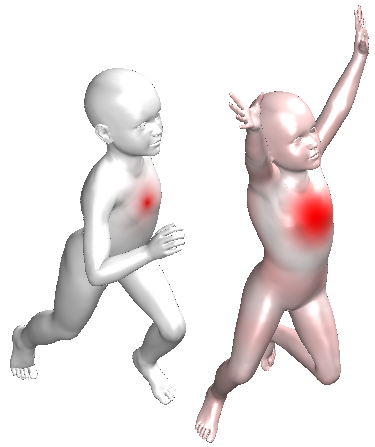
\includegraphics[height=0.4\textwidth]{figs/shape_matching2.png}
  %\caption{CPD Algorithm: $P$ is $M \times N$}
\end{figure}

}


\section{3D Shape Matching}
\frame{
\frametitle{3D Shape Matching}


\begin{figure}
  \centering
    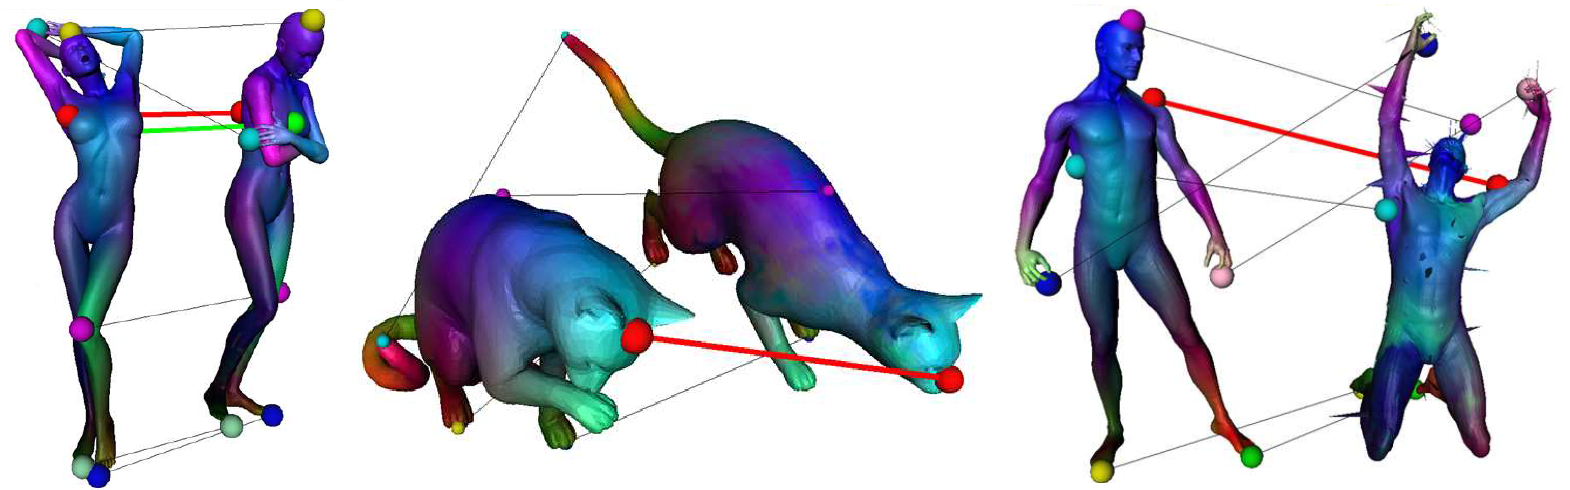
\includegraphics[width=0.65\textwidth]{figs/1.png}
  \caption{Finding Correspondence Between Shapes}
\end{figure}

\begin{figure}
  \centering
    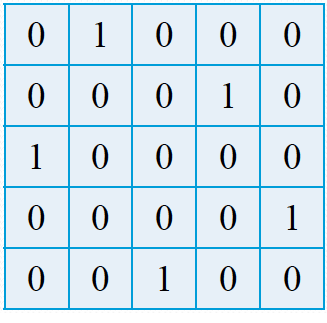
\includegraphics[width=0.25\textwidth]{figs/1_2.png}
  \caption{Correspondence Matrix}
\end{figure}
}

\frame{
\frametitle{3D Shape Matching}


\begin{figure}
  \centering
    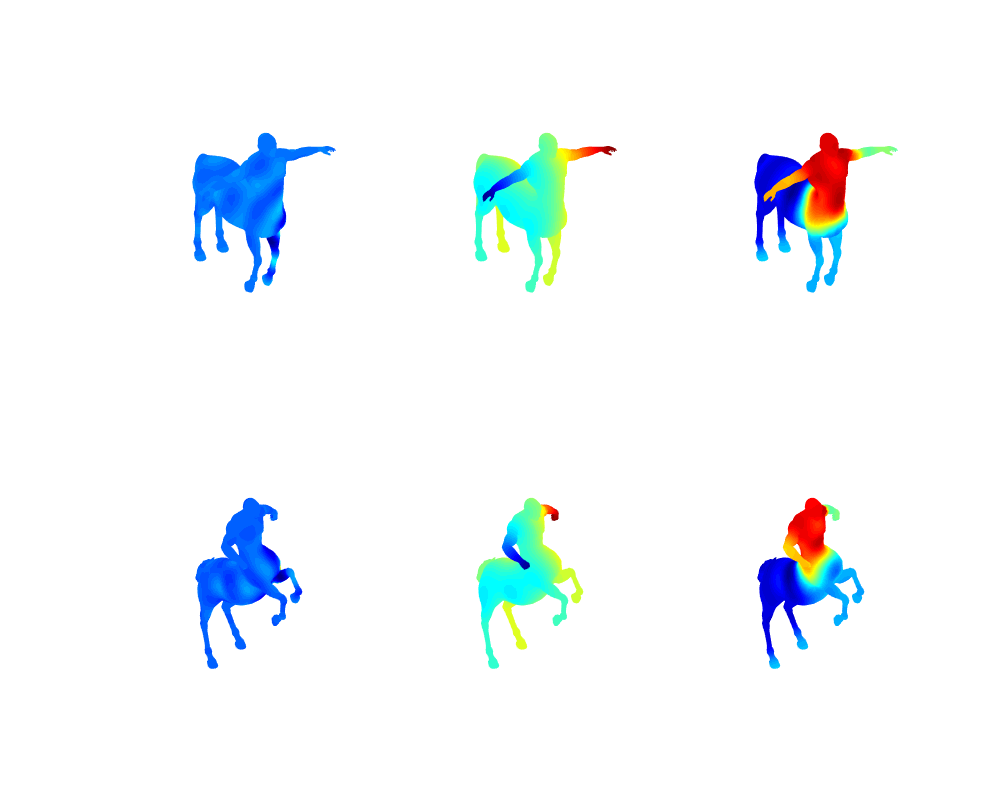
\includegraphics[width=0.75\textwidth]{figs/2.png}
  \caption{Functional Mapping}
\end{figure}

}

\frame{
\frametitle{3D Shape Matching}


\begin{figure}
  \centering
    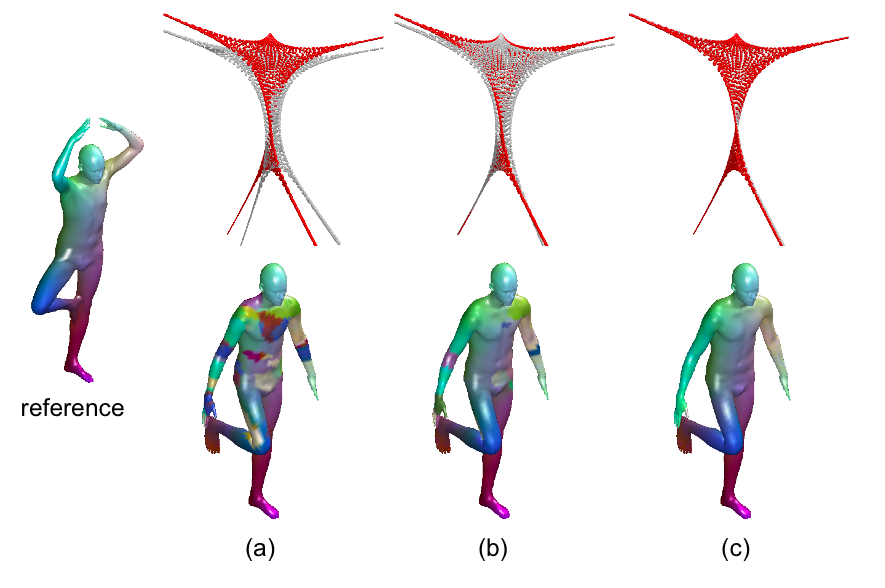
\includegraphics[width=0.65\textwidth]{figs/3.png}
  \caption{Point-To-Point Recovery}
\end{figure}

}



\section{Implementation and Evaluation}
\frame{
\frametitle{Coherent Point Drift (CPD) - Algorithm}

\begin{figure}[h!]
  \centering
    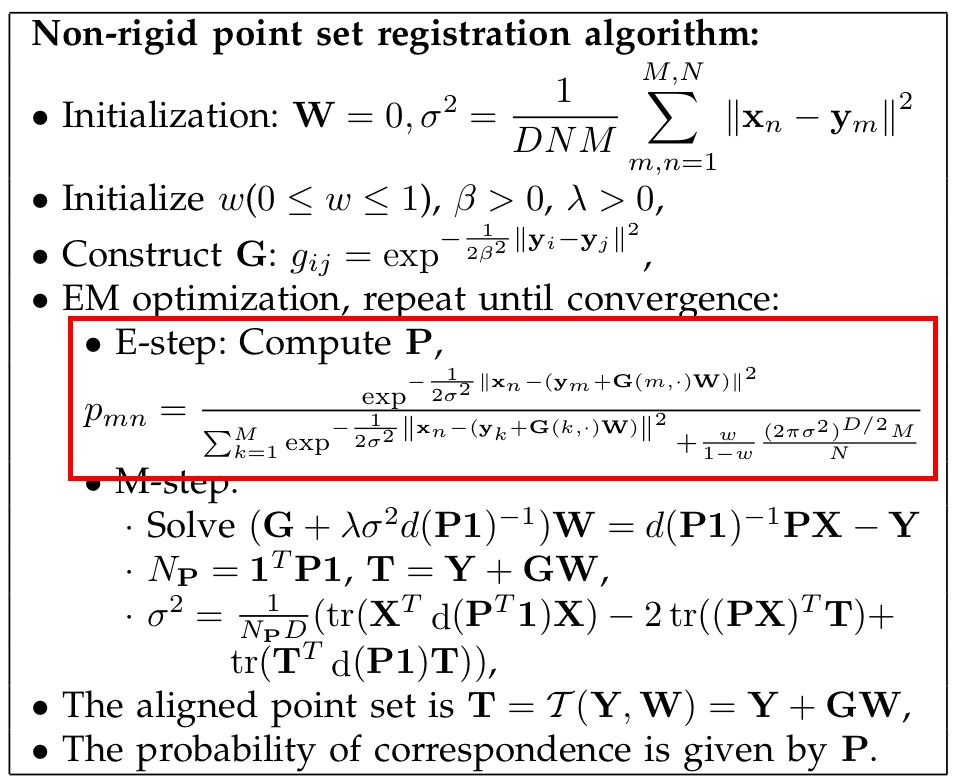
\includegraphics[width=0.7\textwidth]{figs/CPD_P.png}
  \caption{CPD Algorithm: $P$ is $M \times N$ \cite{myronenko2010point}}
\end{figure}

}

\frame{
\frametitle{Coherent Point Drift (CPD) - Implementation}
%\begin{columns}
%\column[t]{0.45\linewidth}
\begin{itemize}
  \item Algorithm
  \begin{itemize}
    \item CPU version uses several loops
    \item Matrix $P$ ($M \times N$) is never actually calculated
  \end{itemize}
  \item GPU Implementation 
  \begin{itemize}
    \item Utilize optimized libraries (CuBLAS)
    \item Vectorize operations
    \item Use matrix slicing to circumvent memory limitations
  \end{itemize}
\end{itemize}
%\begin{figure}[h!]
 % \caption{A picture of a gull.}
 % \centering
%    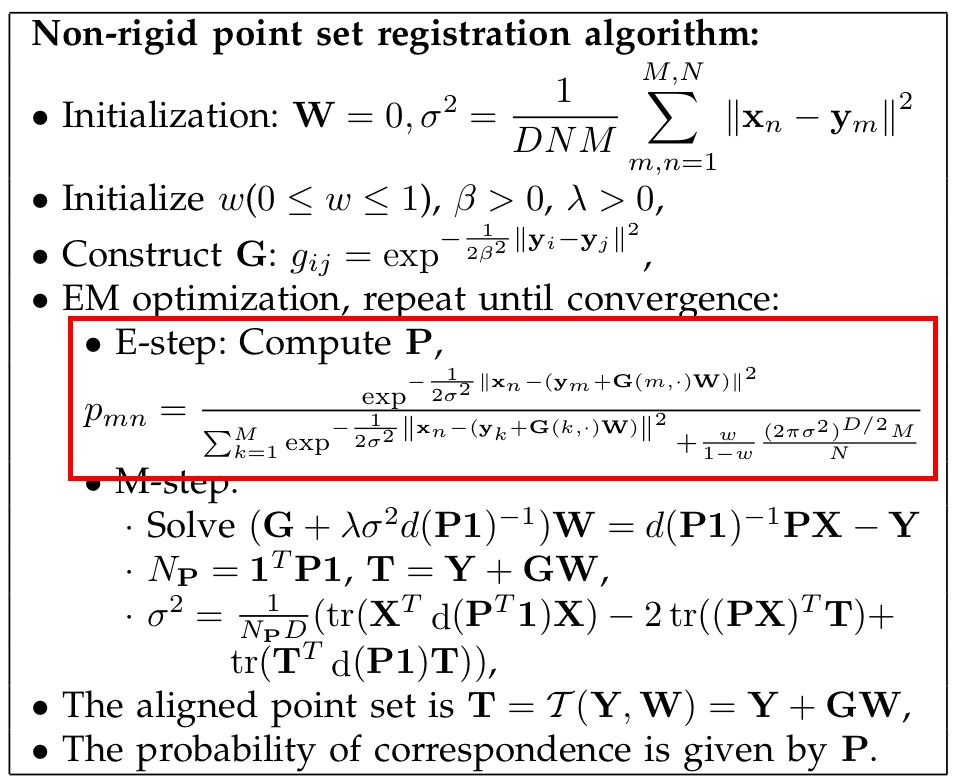
\includegraphics[width=0.5\textwidth]{figs/CPD_P.png}
%\end{figure}
%\column[t]{0.45\linewidth}
%
%\end{columns}

}

\frame{
\frametitle{Coherent Point Drift (CPD) -Evaluation}

\begin{figure}
  \centering
  \subfloat[\label{fig:a}]{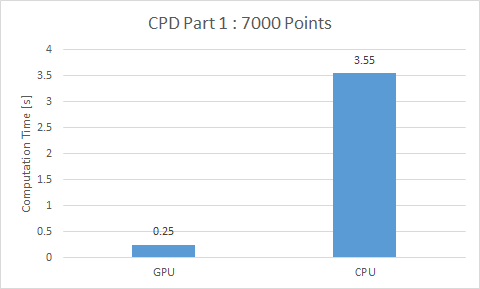
\includegraphics[width=0.45\textwidth]{figs/CPD_P_7k.png}}\qquad    
  \subfloat[\label{fig:b}]{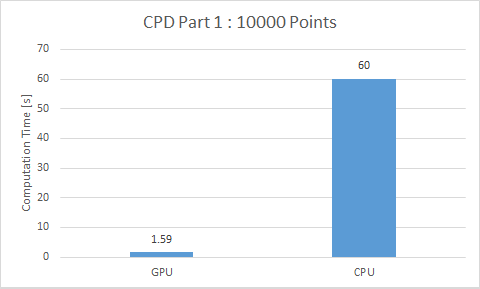
\includegraphics[width=0.45\textwidth]{figs/CPD_P_10k.png}}
  \centering
\caption{Average Runtime for 7000 and 10000 Points}
\label{fig:2}
\end{figure}
    %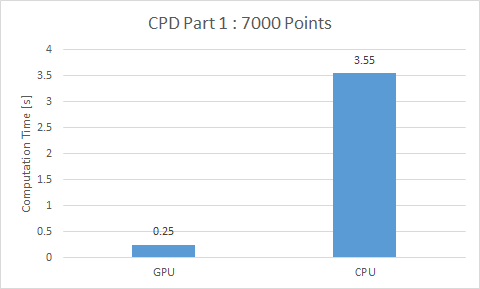
\includegraphics[width=0.4\textwidth]{figs/CPD_P_7k.png}
    %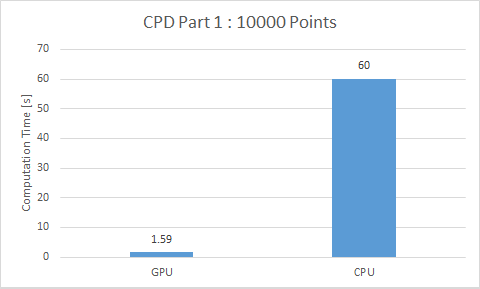
\includegraphics[width=0.4\textwidth]{figs/CPD_P_10k.png}

%\begin{figure}
%  \centering
%    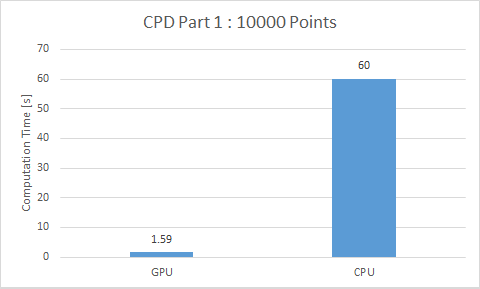
\includegraphics[width=0.4\textwidth]{figs/CPD_P_10k.png}
%\end{figure}
}

\section{Linear System Solver}
\frame{
\frametitle{Linear System Solver}

\begin{itemize}
  \item Large, Dense Linear System of Equations (LSE)
  \item Memory Limitations 
  \item Libraries and approaches (CuSolver, CULA, MAGMA, CuBLAS, Matlab)

\end{itemize}
}

\frame{
\frametitle{Linear System Solver - Evaluation}
\begin{figure}[h!]
  \centering
    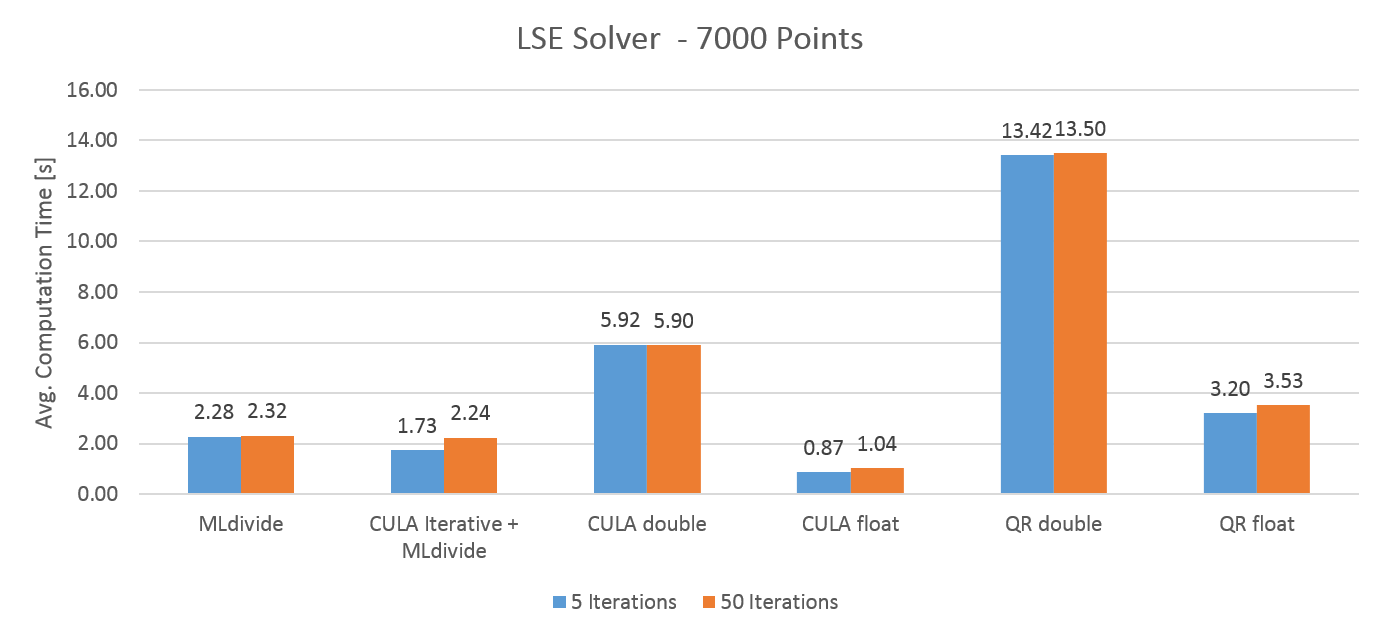
\includegraphics[height=0.5\textwidth]{figs/LSE_comparison_7k.png}
  %\caption{CPD Algorithm: $P$ is $M \times N$}
\end{figure}

    %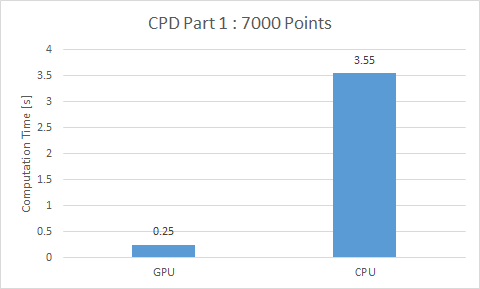
\includegraphics[width=0.4\textwidth]{figs/CPD_P_7k.png}
    %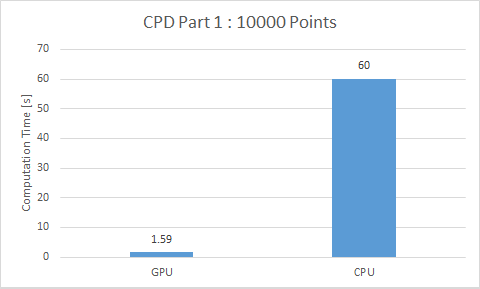
\includegraphics[width=0.4\textwidth]{figs/CPD_P_10k.png}

%\begin{figure}
%  \centering
%    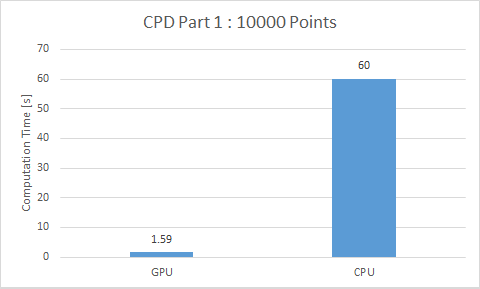
\includegraphics[width=0.4\textwidth]{figs/CPD_P_10k.png}
%\end{figure}
}


%\section{Linear System Solver}
%\frame{
%\frametitle{Coherent Point Drift}

%\begin{itemize}
%  \item Quantitative Evaluation,
%  \begin{itemize}
%%    \item Matching of 7000 Points on CPU: 4.3s
 %   \item GPU Implementation: 0.25s (double precision)
%    \item GPU Implementation: 0.07s (float precision)
%  \end{itemize}
%  \item Qualitative Evaluation,
%  \begin{itemize}
%    \item Double Precision: Exact match with cpu version
%    \item GPU Implementation: 0.25s
%  \end{itemize}
%\end{itemize}
%}

\frame{
\frametitle{Total Runtime}
\begin{figure}[h!]
  \centering
    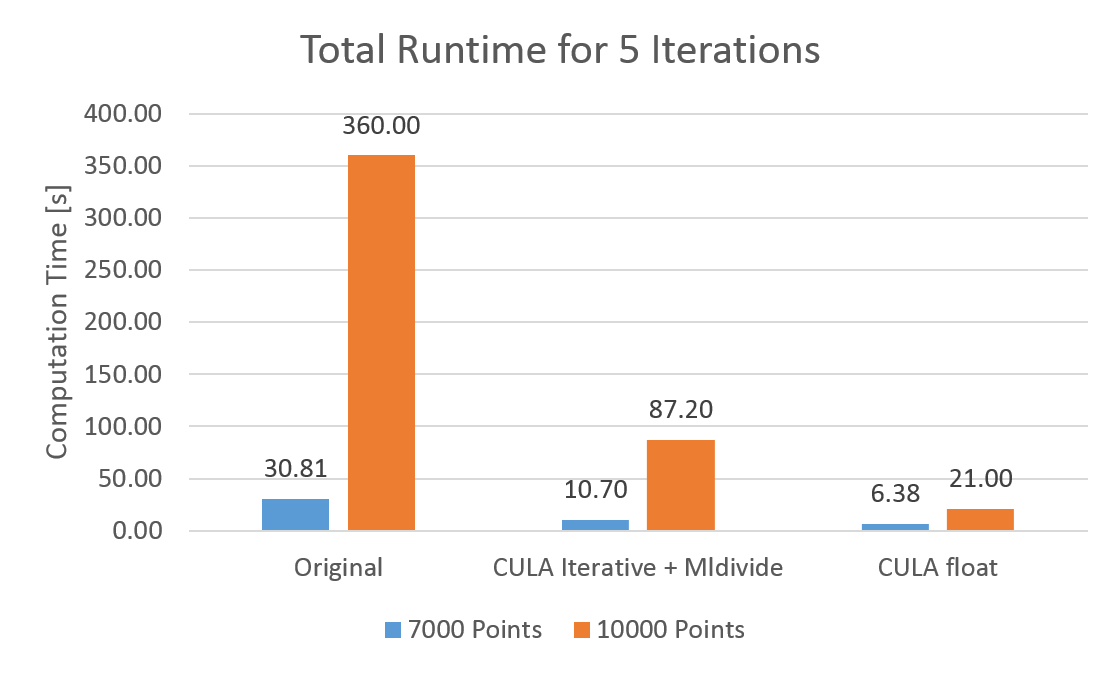
\includegraphics[height=0.55\textwidth]{figs/total_runtimes.png}
  %\caption{CPD Algorithm: $P$ is $M \times N$}
\end{figure}
}

%\section{Demo}
%\frame{
%\frametitle{Demo}
%
%}





\section{Conclusion and Future Work}


\frame{
\frametitle{Conclusion and Future Work}

\begin{itemize}
  \item Consider single precision for whole computation
  \begin{itemize}
    \item Current implementation relies on double precision in CPD
  \end{itemize}
  \item Utilize the new GPU Cluster at the Vision Chair
  \item Develop approach that does not rely on huge, dense LSE
\end{itemize}
}

\frame[allowframebreaks]{
\frametitle{Bibliography}
	\tiny
	\bibliography{bibliography} 
}

\end{document}
